\documentclass[aspectratio=169, table]{beamer}

\usepackage{colortbl}
\usepackage{xcolor}
\usepackage{listings}
\usepackage{tikz}
\usepackage{pgfplots}
\usepgfplotslibrary{polar}
\usetikzlibrary{arrows.meta, positioning, calc}

\usetheme{Pradita}


\usepackage{listings}
\lstdefinestyle{SqlStyle}{
language=SQL,
basicstyle=\ttfamily\footnotesize,
morekeywords={REAL, TEXT, REFERENCES},
keywordstyle=\color{blue},
commentstyle=\color{gray},
stringstyle=\color{red},
breaklines=true,
showstringspaces=false,
tabsize=2,
captionpos=b,
numbers=left,
numberstyle=\tiny\color{gray},
frame=lines,
backgroundcolor=\color{lightgray!10},
comment=[l]{//},
morecomment=[s]{/*}{*/},
commentstyle=\color{gray}\ttfamily,
string=[s]{'}{'},
morestring=[s]{"}{"},
%	stringstyle=\color{teal}\ttfamily,
%	showstringspaces=false
}

\lstdefinelanguage{bash} {
keywords={},
basicstyle=\ttfamily\small,
keywordstyle=\color{blue}\bfseries,
ndkeywords={iex},
ndkeywordstyle=\color{purple}\bfseries,
sensitive=true,
commentstyle=\color{gray},
stringstyle=\color{red},
numbers=left,
numberstyle=\tiny\color{gray},
breaklines=true,
frame=lines,
backgroundcolor=\color{lightgray!10},
tabsize=2,
comment=[l]{\#},
morecomment=[s]{/*}{*/},
commentstyle=\color{gray}\ttfamily,
stringstyle=\color{purple}\ttfamily,
showstringspaces=false
}

% Define Java language style for listings
\lstdefinestyle{JavaScript}{
	language=Java,
	basicstyle=\ttfamily\footnotesize,
	keywordstyle=\color{blue},
	commentstyle=\color{gray},
	stringstyle=\color{red},
	breaklines=true,
	showstringspaces=false,
	tabsize=4,
	captionpos=b,
	numbers=left,
	numberstyle=\tiny\color{gray},
	frame=lines,
	backgroundcolor=\color{lightgray!10},
	comment=[l]{//},
	morecomment=[s]{/*}{*/},
	commentstyle=\color{gray}\ttfamily,
	string=[s]{'}{'},
	morestring=[s]{"}{"},
	%	stringstyle=\color{teal}\ttfamily,
	%	showstringspaces=false
}

\title{\Huge Intro to Unsupervised \\
\vspace{10pt}
Machine Learning}
\subtitle{IT140704 - Big Data for Business}
%\date[Serial]{Penggunaan Large Language Model untuk Pengajaran}
\author{\textbf{Alfa Yohannis}}
\begin{document}

\frame{\titlepage}


\begin{frame}[fragile]
\frametitle{Contents}
\vspace{20pt}
\begin{columns}[t]
	\column{0.5\textwidth}
	\tableofcontents[sections={1-5}]
	
	\column{0.5\textwidth}
	\tableofcontents[sections={6-20}]
\end{columns}
\end{frame}

\begin{frame}{\hfill}
	\centering
	\Huge{\textbf{How can data be used to create real strategic, tactical, and operational values?}}
\end{frame}


\section{Introduction to Unsupervised Learning}

\begin{frame}{Introduction to Unsupervised Learning}
	Unsupervised Learning is used when data has no labels. The model automatically discovers hidden patterns, structures, or segments within the data.
	
	\textbf{Common applications:}
	\begin{itemize}
		\item Customer segmentation based on behavior or demographics.
		\item Anomaly detection in suspicious transactions.
		\item Dimensionality reduction for easier data visualization.
	\end{itemize}
	
	This approach is ideal for early data exploration when labels are unavailable, helping organizations uncover new insights from large and complex datasets.
\end{frame}



\section{Clustering: Automatic Segmentation Without Labels}

\begin{frame}{\LARGE{Clustering: Automatic Segmentation Without Labels}}
	Clustering is an unsupervised learning technique that groups data into clusters based on similarity. Without predefined labels, the algorithm automatically identifies patterns to form homogeneous groups.
	
	\textbf{Business Applications:}
	\begin{itemize}
		\item Customer segmentation based on behavior or demographics.
		\item Personalized service offerings per customer group.
		\item Identifying product usage patterns among users.
		\item Market analysis by grouping geographic areas.
	\end{itemize}
	
	Clustering enables data-driven segmentation that improves marketing efficiency and supports better business decisions.
\end{frame}

\begin{frame}{Clustering Illustration in 2D Space}
	\vspace{20pt}
	\begin{figure}
		\centering
		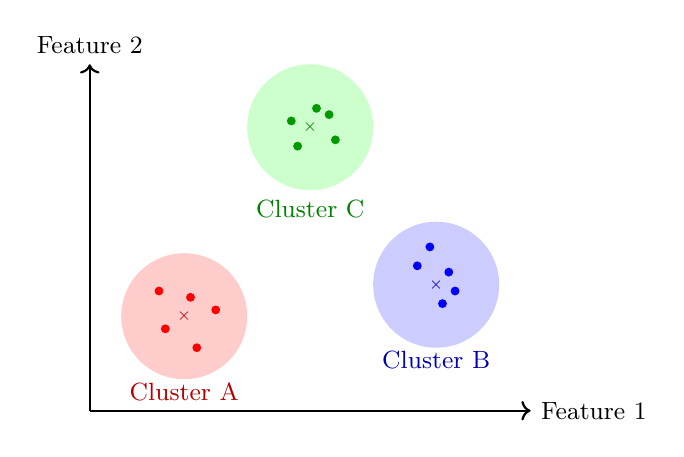
\begin{tikzpicture}[scale=.8]
			
			% Cluster A - Red
			\fill[red!20] (0,0) circle (1);
			\foreach \x/\y in {0.1/0.3, -0.3/-0.2, 0.2/-0.5, -0.4/0.4, 0.5/0.1} {
				\fill[red] (\x,\y) circle (2pt);
			}
			\node[red!70!black] at (0, -1.2) {\small Cluster A};
			\node[red!70!black] at (0, 0) {\tiny $\times$};
			
			% Cluster B - Blue
			\fill[blue!20] (4,0.5) circle (1);
			\foreach \x/\y in {3.7/0.8, 4.1/0.2, 4.2/0.7, 3.9/1.1, 4.3/0.4} {
				\fill[blue] (\x,\y) circle (2pt);
			}
			\node[blue!70!black] at (4, -0.7) {\small Cluster B};
			\node[blue!70!black] at (4, 0.5) {\tiny $\times$};
			
			% Cluster C - Green
			\fill[green!20] (2,3) circle (1);
			\foreach \x/\y in {1.8/2.7, 2.3/3.2, 2.1/3.3, 1.7/3.1, 2.4/2.8} {
				\fill[green!60!black] (\x,\y) circle (2pt);
			}
			\node[green!50!black] at (2, 1.7) {\small Cluster C};
			\node[green!50!black] at (2, 3) {\tiny $\times$};
			
			% Axes
			\draw[->, thick] (-1.5, -1.5) -- (5.5, -1.5) node[right] {\small Feature 1};
			\draw[->, thick] (-1.5, -1.5) -- (-1.5, 4) node[above] {\small Feature 2};
			
		\end{tikzpicture}
		\caption{Illustration of clustering in 2D feature space with three distinct groups and centroids}
		\label{fig:clustering-tikz}
	\end{figure}
\end{frame}


\section{Clustering: Automatic Segmentation Without Labels}

\begin{frame}{K-Means Clustering}
	K-Means is a clustering algorithm that partitions data into \(k\) groups based on average distance to cluster centers (centroids).
	
	\textbf{Steps:}
	\begin{enumerate}
		\item Choose number of clusters \(k\)
		\item Initialize centroids randomly
		\item Assign each point to the nearest centroid
		\item Recalculate centroids
		\item Repeat until centroids stabilize
	\end{enumerate}
	
	\textbf{Pros:} Fast, simple, scalable  
	\textbf{Cons:} Requires \(k\), sensitive to outliers, assumes spherical clusters
\end{frame}

\begin{frame}{k-means Clustering (Iteration Illustration)}
	\vspace{20pt}
	\begin{figure}
		\centering
		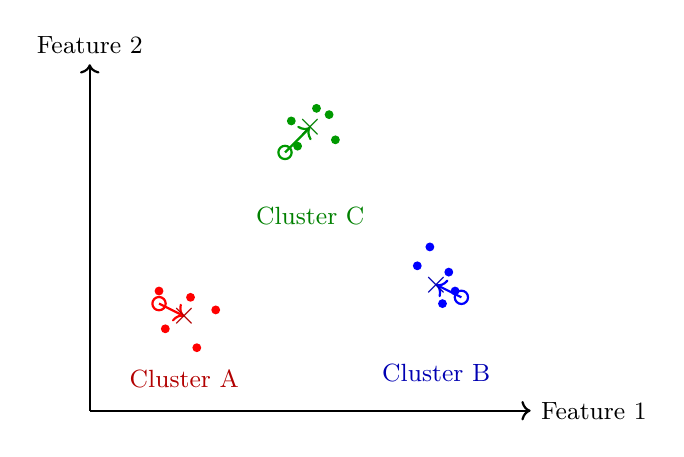
\begin{tikzpicture}[scale=.8]
			
			% ---------- Cluster A (red) ----------
			% points
			\foreach \x/\y in {0.1/0.3, -0.3/-0.2, 0.2/-0.5, -0.4/0.4, 0.5/0.1} {
				\fill[red] (\x,\y) circle (2pt);
			}
			% old centroid (hollow) and new centroid (x), with update arrow
			\draw[red,thick] (-0.4,0.2) circle (3pt);
			\draw[->,red,thick] (-0.4,0.2) -- (0,0);
			\node[red!70!black] at (0,0) {\large $\times$};
			\node[red!70!black] at (0,-1.0) {\small Cluster A};
			
			% ---------- Cluster B (blue) ----------
			\foreach \x/\y in {3.7/0.8, 4.1/0.2, 4.2/0.7, 3.9/1.1, 4.3/0.4} {
				\fill[blue] (\x,\y) circle (2pt);
			}
			\draw[blue,thick] (4.4,0.3) circle (3pt);
			\draw[->,blue,thick] (4.4,0.3) -- (4,0.5);
			\node[blue!70!black] at (4,0.5) {\large $\times$};
			\node[blue!70!black] at (4,-0.9) {\small Cluster B};
			
			% ---------- Cluster C (green) ----------
			\foreach \x/\y in {1.8/2.7, 2.3/3.2, 2.1/3.3, 1.7/3.1, 2.4/2.8} {
				\fill[green!60!black] (\x,\y) circle (2pt);
			}
			\draw[green!60!black,thick] (1.6,2.6) circle (3pt);
			\draw[->,green!60!black,thick] (1.6,2.6) -- (2,3);
			\node[green!50!black] at (2,3) {\large $\times$};
			\node[green!50!black] at (2,1.6) {\small Cluster C};
			
%			% ---------- (Optional) rough Voronoi-style separators ----------
%			% These are illustrative dashed dividers between centroids.
%			\draw[gray!70,dashed] (2,-1.5) -- (2,3.8);   % approx between A (0,0) and B (4,0.5)
%			\draw[gray!70,dashed,rotate around={35:(2,1.5)}] (2,-1.2) -- (2,4.0); % approx between A and C
%			\draw[gray!70,dashed,rotate around={-25:(3,2)}] (2.2,-1.0) -- (3.8,4.2); % approx between B and C
			
			% ---------- Axes ----------
			\draw[->, thick] (-1.5, -1.5) -- (5.5, -1.5) node[right] {\small Feature 1};
			\draw[->, thick] (-1.5, -1.5) -- (-1.5, 4) node[above] {\small Feature 2};
			
		\end{tikzpicture}
		\caption{k-means clustering with $k=3$: points are assigned to the nearest centroid; centroids (×) are updated to the mean of their assigned points (arrows show movement from previous centroids ○).}
		\label{fig:kmeans-tikz}
	\end{figure}
\end{frame}


\begin{frame}{Hierarchical Clustering}
	Hierarchical clustering builds a tree-like structure (dendrogram) to group data based on distance.
	
	\textbf{Approaches:}
	\begin{itemize}
		\item \textbf{Agglomerative:} Start with individual points, merge upward
	\end{itemize}
	
	\textbf{Pros:} No need to set number of clusters, useful for visualizing group structure  
	\textbf{Cons:} Inefficient on large datasets, not easily updated
\end{frame}

\begin{frame}{Hierarchical Clustering Dendrogram}
	\vspace{15pt}
	\begin{figure}
		\centering
		\begin{tikzpicture}[scale=1.5, font=\small]
			% merge heights
			\def\hAB{0.8}\def\hCD{0.9}\def\hEF{0.5}\def\hABCD{1.6}\def\hALL{2.3}
			
			% leaves (x positions)
			\node (A) at (0,-0.2) {A};
			\node (B) at (1.2,-0.2) {B};
			\node (C) at (2.4,-0.2) {C};
			\node (D) at (3.6,-0.2) {D};
			\node (E) at (4.8,-0.2) {E};
			\node (F) at (6.0,-0.2) {F};
			
			% AB merge
			\draw (0,0) -- (0,\hAB);
			\draw (1.2,0) -- (1.2,\hAB);
			\draw (0,\hAB) -- (1.2,\hAB);
			\draw (0.6,\hAB) -- (0.6,\hABCD);   % midpoint up
			
			% CD merge
			\draw (2.4,0) -- (2.4,\hCD);
			\draw (3.6,0) -- (3.6,\hCD);
			\draw (2.4,\hCD) -- (3.6,\hCD);
			\draw (3.0,\hCD) -- (3.0,\hABCD);   % midpoint up
			
			% connect AB and CD at \hABCD
			\draw (0.6,\hABCD) -- (3.0,\hABCD);
			\draw (1.8,\hABCD) -- (1.8,\hALL);  % midpoint up to next level
			
			% EF merge
			\draw (4.8,0) -- (4.8,\hEF);
			\draw (6.0,0) -- (6.0,\hEF);
			\draw (4.8,\hEF) -- (6.0,\hEF);
			\draw (5.4,\hEF) -- (5.4,\hALL);    % midpoint up
			
			% final merge at \hALL
			\draw (1.8,\hALL) -- (5.4,\hALL);
			
			% cut line
			\draw[red,dashed] (-0.4,1.1) -- (6.4,1.1);
			
			% y-axis label
			\node[rotate=90, anchor=south] at (-0.9,1.15) {\small Dissimilarity};
		\end{tikzpicture}
		\caption{Example dendrogram showing merge heights }
		\label{fig:hierarchical-dendrogram}
	\end{figure}
\end{frame}



\begin{frame}{DBSCAN Clustering}
	DBSCAN groups data based on density, not distance. Points with sufficient neighbors form a cluster; isolated points are marked as noise.
	
	\textbf{Key features:}
	\begin{itemize}
		\item Finds clusters of arbitrary shape
		\item Detects outliers automatically
	\end{itemize}
	
	\textbf{Pros:} No need to set \(k\), handles irregular shapes, robust to noise
	 
	\textbf{Cons:} Sensitive to parameters, struggles with high-dimensional data
\end{frame}

\begin{frame}{DBSCAN: Core, Border, and Noise}
	\vspace{20pt}
	\begin{figure}
		\centering
		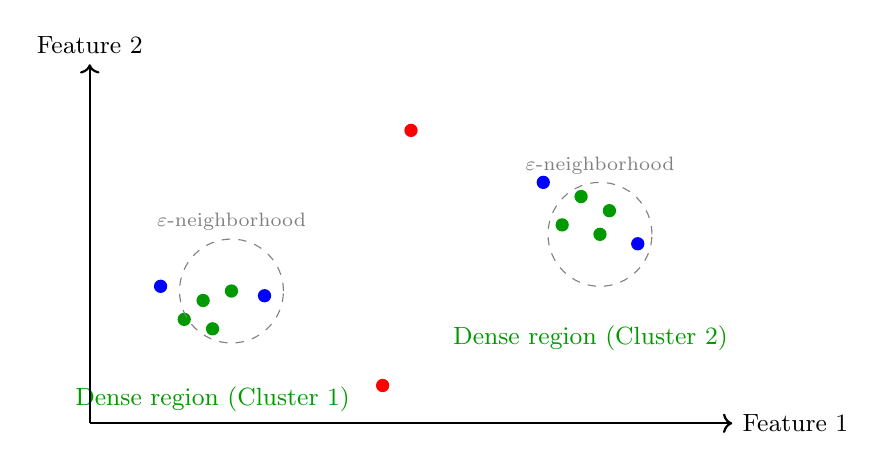
\begin{tikzpicture}[scale=1.2]
			
			% ----- Parameters -----
			\def\eps{0.55} % epsilon radius for illustration
			
			% ----- Cluster A (left) -----
			% Core points (green)
			\fill[green!60!black] (-0.1,0.1) circle (2pt);
			\fill[green!60!black] (0.2,0.2)  circle (2pt);
			\fill[green!60!black] (0.0,-0.2) circle (2pt);
			\fill[green!60!black] (-0.3,-0.1) circle (2pt);
			
			% Border points (blue) near the edge of density
			\fill[blue] (0.55,0.15)  circle (2pt);
			\fill[blue] (-0.55,0.25) circle (2pt);
			
			% Show one epsilon-neighborhood around a core point
			\draw[gray,dashed] (0.2,0.2) circle (\eps);
			
			% Label cluster A
			\node[green!60!black] at (0,-0.95) {\small Dense region (Cluster 1)};
			
			% ----- Cluster B (right) -----
			% Core points (green)
			\fill[green!60!black] (3.7,0.9) circle (2pt);
			\fill[green!60!black] (4.1,0.8) circle (2pt);
			\fill[green!60!black] (3.9,1.2) circle (2pt);
			\fill[green!60!black] (4.2,1.05) circle (2pt);
			
			% Border points (blue)
			\fill[blue] (4.5,0.7) circle (2pt);
			\fill[blue] (3.5,1.35) circle (2pt);
			
			% Epsilon circle for one core point
			\draw[gray,dashed] (4.1,0.8) circle (\eps);
			
			% Label cluster B
			\node[green!60!black] at (4.0,-0.3) {\small Dense region (Cluster 2)};
			
			% ----- Noise points (red) -----
			\fill[red] (2.1, 1.9) circle (2pt);
			\fill[red] (1.8,-0.8) circle (2pt);
			
			% ----- Axes -----
			\draw[->, thick] (-1.3, -1.2) -- (5.5, -1.2) node[right] {\small Feature 1};
			\draw[->, thick] (-1.3, -1.2) -- (-1.3, 2.6) node[above] {\small Feature 2};
			
			% ----- Legend -----
			\begin{scope}[shift={(2.6,2.1)}]
%				\draw[rounded corners, gray!40] (-0.2,-0.35) rectangle (3.0,0.45);
%				\fill[green!60!black] (0,0) circle (2pt);
%				\node[anchor=west] at (0.1,0.3) {\small Core point};
%				\fill[blue] (1.3,0) circle (2pt);
%				\node[anchor=west] at (1.5,0) {\small Border point};
%				\fill[red] (2.6,0) circle (2pt);
%				\node[anchor=west] at (2.8,0) {\small Noise};
			\end{scope}
			
			% Label epsilon
			\node[gray] at (0.2,0.2+\eps+0.18) {\scriptsize $\varepsilon$-neighborhood};
			\node[gray] at (4.1,0.8+\eps+0.18) {\scriptsize $\varepsilon$-neighborhood};
			
		\end{tikzpicture}
		\caption{DBSCAN illustration: core points (green) have $\ge$ \textit{minPts} neighbors within radius $\varepsilon$; border points (blue) are reachable from a core but not dense; noise (red) lies outside any dense region.}
		\label{fig:dbscan-tikz}
	\end{figure}
\end{frame}


\begin{frame}{Choosing the Right Clustering Method}
	\textbf{Selection depends on:}
	\begin{itemize}
		\item Desired cluster shape and count
		\item Dataset size and dimensionality
		\item Use case: segmentation or anomaly detection
		\item Need for interpretability or visual output
	\end{itemize}
	
	\textbf{Typical Use:}
	\begin{itemize}
		\item \textbf{K-Means:} General-purpose, efficient for large datasets
		\item \textbf{Hierarchical:} Ideal for early exploration and structure discovery
		\item \textbf{DBSCAN:} Great for complex shapes and detecting outliers
	\end{itemize}
\end{frame}


\section{Dimensionality Reduction and Visualization}

\begin{frame}{Visualization: Why Dimensionality Reduction?}
	High-dimensional data (e.g., customer profiles with many attributes) is hard to analyze and visualize. Dimensionality reduction simplifies the data while preserving essential information.
	
	\textbf{Key benefits:}
	\begin{itemize}
		\item \textbf{Visualization:} Enables 2D or 3D mapping of complex data.
		\item \textbf{Noise reduction:} Removes irrelevant or redundant features.
		\item \textbf{Efficiency:} Reduces computation time for model training.
		\item \textbf{Avoids dimensionality curse:} Helps models find meaningful patterns.
	\end{itemize}
	
	It is essential for exploring and analyzing big data effectively.
\end{frame}

\begin{frame}{PCA: Principal Component Analysis}
	PCA is a linear technique that transforms original features into new variables called principal components, ordered by their contribution to data variance.
	
	\textbf{Pros:}
	\begin{itemize}
		\item Computationally efficient
		\item Interpretable
		\item Suitable for numeric, linear data
	\end{itemize}
	
	\textbf{Cons:}
	\begin{itemize}
		\item Cannot capture non-linear patterns
		\item Reduced dimensions are hard to map back to original features
	\end{itemize}
	
	\textbf{Business use:} Simplify customer survey data into key satisfaction drivers.
\end{frame}

%\begin{frame}{t-SNE: For Cluster Visualization}
%	t-SNE is a non-linear technique for visualizing high-dimensional data in 2D or 3D by preserving local similarities between data points.
%	
%	\textbf{Pros:}
%	\begin{itemize}
%		\item Excellent for visualizing clusters
%		\item Captures non-linear structures
%	\end{itemize}
%	
%	\textbf{Cons:}
%	\begin{itemize}
%		\item Not scalable for large datasets
%		\item Not suited for training pipelines
%		\item Results may vary across runs
%	\end{itemize}
%	
%	\textbf{Business use:} Visualize customer segments for intuitive analysis.
%\end{frame}
%
%\begin{frame}{PCA vs. t-SNE: Summary}
%	\textbf{Comparison Overview:}
%	\begin{itemize}
%		\item \textbf{PCA:} Linear, scalable, reproducible; used for preprocessing and analysis.
%		\item \textbf{t-SNE:} Non-linear, great for visual clustering, less consistent across runs.
%	\end{itemize}
%	
%	\textbf{Use in Business:}
%	\begin{itemize}
%		\item PCA simplifies complex datasets into core dimensions.
%		\item t-SNE helps stakeholders understand customer clusters visually.
%	\end{itemize}
%	
%	Dimensionality reduction boosts both insight and efficiency in modern data workflows.
%\end{frame}

\section{Customer Segmentation with Clustering}

\begin{frame}{Why Segment Customers?}
	Clustering is widely used in business to divide customers into distinct groups based on similarities in behavior or characteristics. 
	
	Rather than treating all customers the same, segmentation enables personalized marketing, improved service, and more efficient resource allocation. 
	
	Clustering is especially helpful for companies with large and diverse customer bases. By identifying segments automatically, businesses can develop more relevant, targeted, and data-driven strategies to increase retention, boost satisfaction, and reduce wasted marketing effort.
\end{frame}

\begin{frame}{Case Study: Online Store Segmentation}
	An online store analyzes historical transaction data to segment customers using key features:
	
	\begin{itemize}
		\item \textbf{Recency} – days since last purchase
		\item \textbf{Frequency} – number of purchases
		\item \textbf{Monetary} – total spending
	\end{itemize}
	
	These RFM metrics are widely used for customer behavior analysis. Data is normalized to avoid scale bias. 
	
	\textbf{K-Means Clustering} is applied with \(k = 4\) clusters, selected via the elbow method to balance grouping clarity and model simplicity.
\end{frame}

\begin{frame}{Clustering Results: Four Customer Groups}
	The analysis yields 4 distinct clusters:
	
	\begin{itemize}
		\item \textbf{Loyal Customers:} High frequency and spending, recently active.
		\item \textbf{Potential Loyalists:} Moderate activity, recent transactions.
		\item \textbf{Passive Customers:} Rare activity, low spending, inactive.
		\item \textbf{Price-Sensitive:} Frequent buyers with low transaction value.
	\end{itemize}
	
	These groups enable tailored actions: loyalty rewards for Cluster A, reactivation campaigns for C, discounts for D, and onboarding for B.
\end{frame}

%\begin{frame}{Visualization and Business Impact}
%	\vspace{20pt}
%	\textbf{Visualization:}
%	\begin{itemize}
%		\item Use \textbf{PCA} or \textbf{t-SNE} to project customers into 2D space
%		\item Helps managers intuitively see patterns and cluster proximity
%	\end{itemize}
%	
%	\vspace{5pt}
%	\textbf{Evaluation:}
%	\begin{itemize}
%		\item Assess cluster quality using metrics like:
%		\begin{itemize}
%			\item \textit{Silhouette Score}
%			\item \textit{Davies-Bouldin Index}
%		\end{itemize}
%	\end{itemize}
%	
%	\vspace{5pt}
%	\textbf{Business Impact:}
%	\begin{itemize}
%		\item Enables data-driven strategies
%		\item Improves personalization and marketing ROI
%		\item Enhances long-term customer understanding
%	\end{itemize}
%\end{frame}


\section{Customer Segmentation with Clustering}

\begin{frame}{Why Segment Customers?}
	Clustering divides customers into groups based on shared behaviors or traits. 
	
	\textbf{Benefits:}
	\begin{itemize}
		\item Enables personalized marketing and service
		\item Improves resource allocation and ROI
		\item Avoids ineffective one-size-fits-all strategies
	\end{itemize}
	
	Especially useful for large, diverse customer bases, clustering helps businesses design targeted, relevant, and cost-effective approaches by leveraging real behavioral patterns instead of assumptions.
\end{frame}

\begin{frame}{Case Study: Online Store Segmentation}
	An online store uses transaction history to cluster customers using:
	
	\begin{itemize}
		\item \textbf{Recency:} Days since last purchase
		\item \textbf{Frequency:} Total number of purchases
		\item \textbf{Monetary:} Total spending amount
	\end{itemize}
	
	This RFM model captures customer value and engagement. Features are normalized, and K-Means is applied with \(k = 4\), selected using the elbow method to balance simplicity and insight.
\end{frame}

\begin{frame}{Clustering Results: Four Segments}
	Clustering yields four meaningful customer segments:
	
	\begin{itemize}
		\item \textbf{Loyal Customers:} High spenders, recent and frequent buyers
		\item \textbf{Potential Loyalists:} Recent activity, moderate value
		\item \textbf{Passive Customers:} Infrequent, low-value, inactive
		\item \textbf{Price-Sensitive:} Frequent small purchases, promo-driven
	\end{itemize}
	
	These segments support specific actions like loyalty programs, reactivation efforts, discount targeting, and onboarding.
\end{frame}

%\begin{frame}{Visualization and Business Impact}
%	\textbf{Visualization:}
%	\begin{itemize}
%		\item Use PCA or t-SNE to map clusters in 2D
%		\item Color-coded points show group distribution
%	\end{itemize}
%	
%	\textbf{Evaluation:}
%	\begin{itemize}
%		\item Silhouette Score and Davies-Bouldin Index assess cluster quality
%	\end{itemize}
%	
%	Clustering reveals actionable insights, supporting better campaign targeting, retention planning, and customer understanding—all grounded in actual data patterns.
%\end{frame}



\section{Customer Clustering Hands-On}

\begin{frame}{Objective of the Hands-On}
	This hands-on session aims to segment customers based on behavior or attributes using the K-Means algorithm.
	
	\begin{itemize}
		\item Perform clustering on customer data
		\item Visualize segments using projection techniques
		\item Analyze segment characteristics to uncover business insights
	\end{itemize}
	
	The goal is to understand how customer segmentation using unsupervised learning can help inform marketing, retention, and personalization strategies.
\end{frame}

\begin{frame}{Dataset Description}
	\vspace{20pt}
	The dataset is in CSV format and includes:
	
	\begin{itemize}
		\item \textbf{Recency}: Days since last transaction
		\item \textbf{Frequency}: Number of purchases
		\item \textbf{Monetary}: Total purchase value
		\item \textbf{Customer ID}: Unique identifier (excluded from clustering)
	\end{itemize}
	
	\textbf{Sources:}
	\begin{itemize}
		\item UCI Online Retail Dataset: \url{https://archive.ics.uci.edu/ml/datasets/Online+Retail}
		\item Cleaned RFM Version: \url{https://u.pcloud.link/publink/show?code=kZ6a7W5Zr4Y3H3bMCSfxrMGxSut20VEohrGk}
	\end{itemize}
	
	Ensure the file \texttt{frm\_results.csv} is available locally before beginning.
\end{frame}

\begin{frame}{Workflow in Orange}
	\textbf{Steps to Build Workflow:}
	
	\begin{enumerate}
		\item Load dataset using \texttt{File}
		\item Preview data with \texttt{Data Table}
		\item Apply \texttt{k-Means}, set \(k = 3\)
		\item View cluster output in \texttt{Data Table}
		\item Use \texttt{Linear Projection} to visualize clusters
		\item Split data by cluster and analyze with \texttt{Statistics}
		\item Use \texttt{Box Plot} for RFM analysis per cluster
	\end{enumerate}
	
	\textit{This visual workflow makes clustering accessible without writing code.}
\end{frame}

\begin{frame}{Workflow Diagram in Orange}
	\begin{figure}
		\centering
		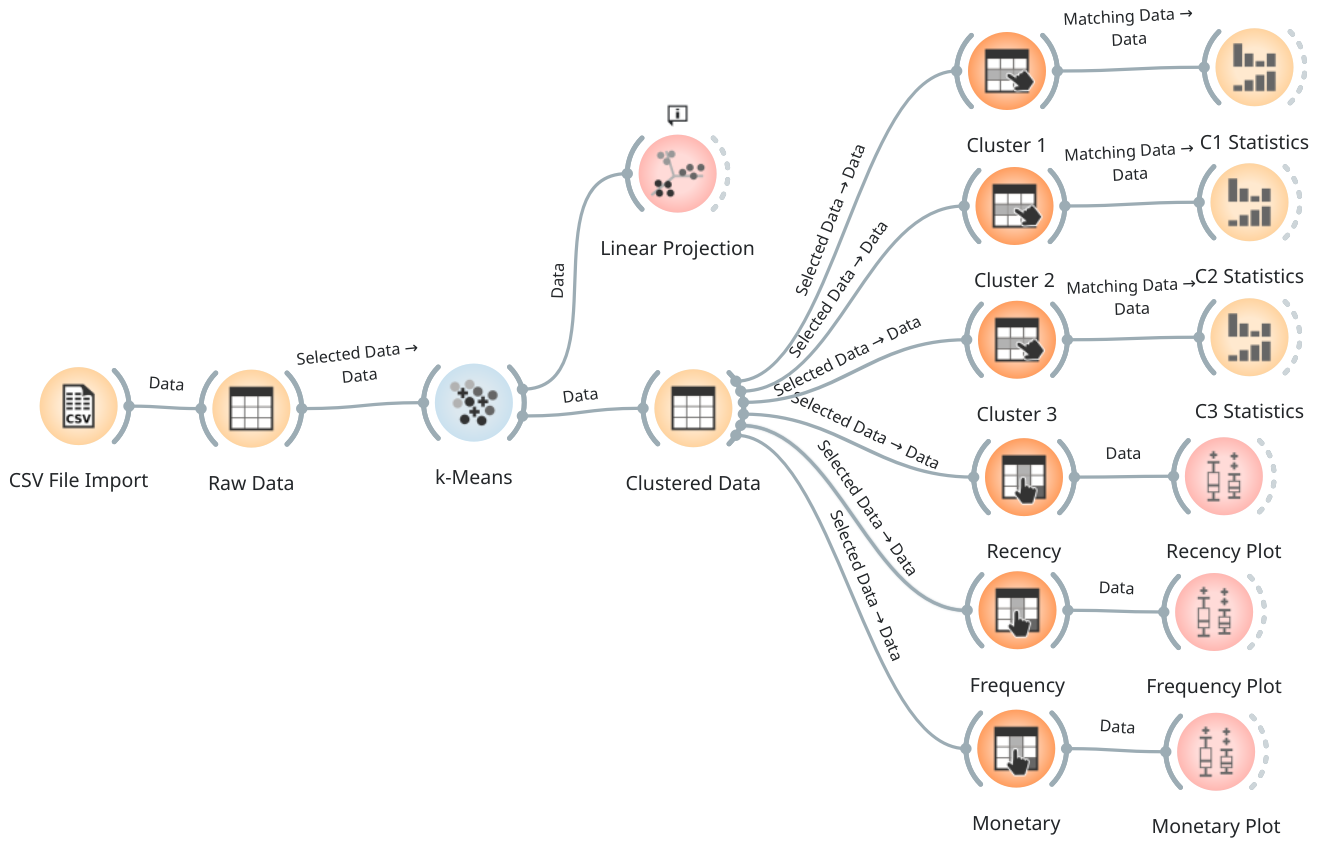
\includegraphics[width=.9\linewidth]{../../figures/clustering.png}
		\caption{Customer segmentation using K-Means in Orange}
		\label{fig:clustering-orange}
	\end{figure}
\end{frame}


\begin{frame}{Result Analysis}
	\textbf{After clustering:}
	
	\begin{itemize}
		\item Observe cluster sizes and composition
		\item Identify characteristics:
		\begin{itemize}
			\item High \texttt{Monetary} → VIP
			\item High \texttt{Recency}, low \texttt{Frequency} → Passive
		\end{itemize}
		\item Use findings to tailor marketing strategies
	\end{itemize}
	
	K-Means shows how customers naturally group by behavior. Visual tools like scatter plots and box plots help interpret these segments intuitively, providing key insights for business decision-making.
\end{frame}

\section{Interpreting Segmentation Results and Business Strategy}

\begin{frame}{Customer Segmentation: 3D Visualization}
	\vspace{20pt}
	\begin{columns}[c]
		\column{0.48\textwidth}
		\small
		This 3D plot shows how customer clusters are distributed in the RFM space:
		\begin{itemize}
			\item \textbf{X-axis:} Recency (days since last purchase)
			\item \textbf{Y-axis:} Frequency (number of purchases)
			\item \textbf{Z-axis:} Monetary (total spend)
		\end{itemize}
		\vspace{4pt}
		The visual separation of clusters helps identify distinct behavioral patterns and verify the clustering quality in three dimensions.
		
		\column{0.52\textwidth}
		\centering
		\fbox{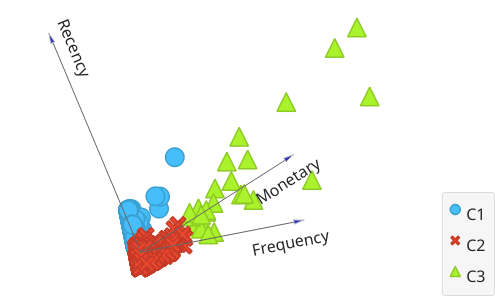
\includegraphics[width=1.02\linewidth]{../../figures/3d_plot.png}}
	\end{columns}
\end{frame}


\begin{frame}{Recency Distribution}
	\vspace{20pt}
	\begin{columns}[c]
		\column{0.48\textwidth}
		\small
		This plot shows the distribution of recency values across customer clusters.  
		\begin{itemize}
			\item Cluster C1 (Dormant Buyers): average recency = 246 days  
			\item Cluster C2 (Regular Shoppers): avg. recency = 41 days  
			\item Cluster C3 (VIP Customers): avg. recency = 6 days  
		\end{itemize}
		High recency indicates inactivity, while low recency suggests recent transactions.
		
		\column{0.52\textwidth}
		\centering
		\fbox{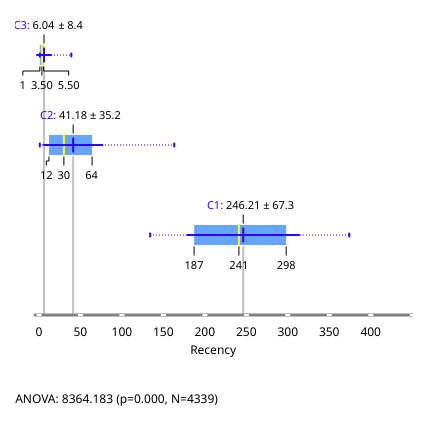
\includegraphics[width=0.9\linewidth]{../../figures/recency.png}}
	\end{columns}
\end{frame}

\begin{frame}{Frequency Distribution}
	\vspace{20pt}
	\begin{columns}[c]
		\column{0.48\textwidth}
		\small
		This chart illustrates how frequently customers from each cluster make purchases.  
		\begin{itemize}
			\item Cluster C1: very low frequency (1.58 purchases)  
			\item Cluster C2: moderate frequency (4.68 purchases)  
			\item Cluster C3: very high frequency (66.5 purchases)  
		\end{itemize}
		Frequency is a key indicator of engagement and retention.
		
		\column{0.52\textwidth}
		\centering
		\fbox{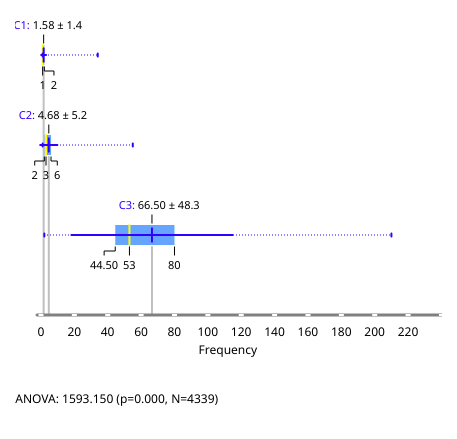
\includegraphics[width=0.9\linewidth]{../../figures/frequency.png}}
	\end{columns}
\end{frame}

\begin{frame}{Monetary Distribution}
	\vspace{20pt}
	\begin{columns}[c]
		\column{0.48\textwidth}
		\small
		This visualization shows the average monetary value spent by each customer cluster.  
		\begin{itemize}
			\item Cluster C1: low spenders (~629)  
			\item Cluster C2: moderate spenders (~1,859)  
			\item Cluster C3: high-value spenders (~85,900)  
		\end{itemize}
		Indicates the revenue contribution potential from each group.
		
		\column{0.52\textwidth}
		\centering
		\fbox{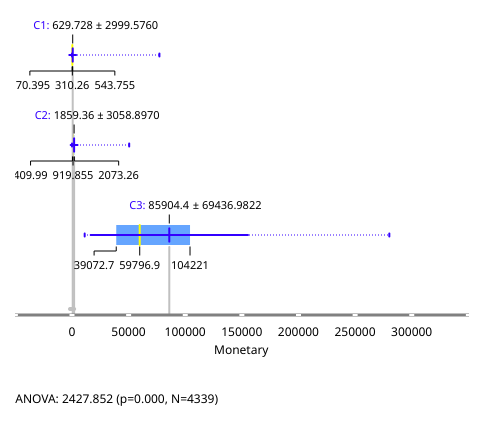
\includegraphics[width=0.85\linewidth]{../../figures/monetary.png}}
	\end{columns}
\end{frame}


\begin{frame}{Cluster Profiles and Labeling}
\vspace{20pt}

K-Means clustering yielded three distinct segments based on RFM data:

\begin{itemize}
\item \textbf{Cluster C1 – \textit{Dormant Buyers}:} Very high recency (246 days), very low frequency (1.58), and low monetary value (629). These are inactive customers with minimal engagement.
\item \textbf{Cluster C2 – \textit{Regular Shoppers}:} Moderate recency (41 days), frequency (4.68), and monetary value (1,859). They are consistent, mid-value customers.
\item \textbf{Cluster C3 – \textit{VIP Customers}:} Very recent activity (6 days), very high frequency (66.5), and high spending (85,900). This group contributes most to revenue.
\end{itemize}

Labels are based on the clear separation in behavioral and transactional metrics.
\end{frame}

\begin{frame}{Strategic Approach by Cluster}
\vspace{20pt}

\textbf{VIP Customers (C3)} should be prioritized:

\begin{itemize}
\item Offer loyalty programs, VIP perks, and early access to new products.
\item Build personal relationships to sustain the 85K+ average spending.

\textbf{Regular Shoppers (C2)} show promise:
\item Encourage upsell via product bundles and point rewards.
\item Target campaigns to move them beyond the 1.8K spending level.

\textbf{Dormant Buyers (C1)} need reactivation:
\item Send “We miss you” campaigns and special return incentives.
\item Explore reasons behind their 246-day inactivity via surveys.
\end{itemize}
\end{frame}

\begin{frame}{Retention and Marketing Efficiency}
\vspace{20pt}

RFM segmentation enables precise targeting and efficient budgeting:

\begin{itemize}
\item \textbf{Cluster C3 (VIP)} deserves high-touch campaigns to protect their high lifetime value and frequent purchases.
\item \textbf{Cluster C1 (Dormant)} can be addressed through automated, low-cost reactivation flows.
\item \textbf{Cluster C2 (Regular)} should receive incentives to shift them into VIP territory.
\end{itemize}

Tracking metrics like churn, repeat rate, and average revenue by segment gives marketers actionable insight and allows continuous optimization.
\end{frame}

\begin{frame}{Conclusion and Next Steps}
\vspace{20pt}

Segmentation is not the end—it guides business decisions forward:

\begin{itemize}
\item Integrate clusters into CRM and email automation tools.
\item Monitor per-cluster KPIs (e.g., VIP revenue share or C1 churn rate).
\item Refine labels as customer behavior shifts.
\end{itemize}

The numbers behind each cluster justify their strategic importance. Acting on them leads to better engagement, smarter resource use, and stronger long-term customer value.
\end{frame}

\begin{frame}{Conclusion}
	\vspace{20pt}
	
	Unsupervised learning helps businesses gain insights from unlabelled data by:
	
	\begin{itemize}
		\item \textbf{Clustering:} uncovering natural groupings (e.g., customer segments).
		\item \textbf{Dimensionality reduction:} simplifying complex data for visualization and modeling.
		\item \textbf{Anomaly detection:} identifying rare or suspicious behaviors.
		\item \textbf{Exploratory analysis:} revealing structure when no labels exist.
	\end{itemize}
	
	These techniques are vital when labels are unavailable or costly. In Big Data contexts, they enable data-driven strategy, personalization, and operational efficiency—transforming raw information into meaningful business value.
\end{frame}


\end{document}
